\documentclass[cn,11pt,chinese]{elegantbook}

\usepackage[all]{xy}
\usepackage{amsmath}
\usepackage{asymptote}
\usepackage{subfig}
\usepackage{graphicx}



\newcount\mycount
\def\cis{\,\text{cis}\,}
\def\intset{\operatorname{int}}
\def\diam{\operatorname{diam}}
\def\dist{\operatorname{dist}}
\def\ulim{\operatorname{u-lim}}
\def\cinfty{\mathbb{C}_{\infty}}
\def\sh{\operatorname{sh}}
\def\argsh{\operatorname{argsh}}
\def\ch{\operatorname{ch}}
\def\argch{\operatorname{argch}}
\def\real{\mathbb{R}}
\def\complex{\mathbb{C}}
\def\dsint{{\displaystyle\int}}

\numberwithin{equation}{section}


% title info
\title{微积分}
\subtitle{第二卷}

% bio info
\author{Tom. M. Apostol}

% extra info
\version{1.00}
\extrainfo{Wir m\"ussen wissen, wir werden wissen. (我们必须知道,我们必将知道) - David.Hilbert}
%\logo{logo.png}
\cover{cover.jpg}

\begin{document}


\maketitle

\chapter*{Preface}


\tableofcontents
\mainmatter
\hypersetup{pageanchor=true}

% add preface chapter here if needed

\part{Linear Analysis}
\chapter{Linear Spaces}
\section{Introduction}
Throughout mathematics we encounter many examples of mathematical objects that can be added to each other and multiplied by real numbers. First of all, the real numbers themselves are such objects. Other examples are real-valued functions, the complex numbers, infinite series, vectors in $n$-space, and vector valued functions. In this chapter we discuss a general mathematical concept, called a linear space, which includes all these examples and many others as special cases.

Briefly, a linear space is a set of elements of any kind on which certain operations (called addition and multiplication by numbers) can be performed. In defining a linear space, we do not specify the nature of the elments nor do we tell how the operations are to be performed on them. Instead, we require that the operations have certain properties which we take as axioms for a linear space. We turn now to a detailed description of these axioms.


\section{The definition of a linear space}
Let $V$ denote a nonempty set of objects, called elements. The set $V$ is called a linear space if it satisfies the following ten axioms which we list in three groups.

Closure axioms

AXIOM 1. CLISURE UNDER ADDITION. For every pair of elements $x$ and $y$ in $V$ there corresponds a unique element in $V$ called the sum of $x$ and $y$, denoted by $x + y$.

AXIOM 2. CLOSURE UNDER MULTIPLICATION BY REAL NUMBERS. For every $x$ in $V$ and every real number $a$ there corresponds an element in $V$ called the product of $a$ and $x$, denoted by $ax$.

Axioms for addition

AXIOM 3. COMMUTATIVE LAW. For all $x$ and $y$ in $V$, we have $x = Y = y + x$.

AXIOM 4. ASSOCIATIVE LAW. For all $x$, $y$ and $z$ in $V$, we have $(x + y) + z = x + (y + z)$.

AXIOM 5. EXISTENCE OF ZERO ELEMENT. There is an element in $V$, denoted by $O$, such that 
\[
x+ O = x \quad \text{for all $x$ in $V$}.
\]

AXIOM 6. EXISTENCE OF NEGATIVES. For every $x$ in $V$, the element $(-1)x$ has the property
\[
x + (-1)x = O.
\]

Axioms for multiplication by numbers

AXIOM 7. ASSOCIATIVE LAW. For every $x$ in $V$ and all real numbers $a$ and $b$, we have 
\[
a(bx) = (ab)x.
\]

AXIOM 8. DISTRIBUTIVE LAW FOR ADDITION IN $V$. For all $x$ and $y$ in $V$ and all real $a$, we have
\[
a(x+y) = ax + ay.
\]

AXIOM 9. DISTRIBUTIVE LAW FOR ADDITION OF NUMBERS. For all $x$ in $V$ and all real $a$ and $b$, we have
\[
(a+b)x = ax + bx.
\]

AXIOM 10. EXISTENCE OF IDENTITY. For every $x$ in $V$, we have $1x = x$.

Linear spaces, as defined above, are sometimes called real linear spaces to emphasize the fact that we are multiplying the elements of $V$ by real numbers. If real number is replaced by complex number in Axioms 2,7,8, and 9, the resulting structure is called a complex linear space. Sometimes a linear space is referred to as a linear vector space or simply a vector space; the numbers used as multipliers are also called scalars. A real linear space has real numbers as scalars; a complex linear space has complex numbers as scalars. Although we shall deal primarily with examples of real linear spaces, all the theorems are valid for complex linear spaces as well. When we use the term linear space without further designation, it is to be understood that the space can be real or complex.

\section{Examples of linear spaces}
If we specify the set $V$ and tell how to add its elements and how to multiply them by numbers, we get a concrete example of a linear space. The reader can easily verify that each of the following examples satisfies all the axioms for a real linear space.

\begin{example}\label{exam020010301}
Let $V = \real$, the set of all real numbers, and let $x + y$ and $ax$ be ordinary addition and multiplication of real numbers.
\end{example}

\begin{example}\label{exam020010302}
Let $V = \complex$, the set of all complex numbers, define $x + y$ to be ordinary addition of complex numbers, and define $ax$ to be multiplication of the complex number $x$ by the real number $a$. Even though the elements of $V$ are complex numbers, this is a real linear space because the scalars are real.
\end{example}

\begin{example}\label{exam020010303}
Let $V = V_n$, the vector space of all $n$-tuples of real numbers, with addition and multiplication by scalars defined in the usual way in terms of components.
\end{example}

\begin{example}\label{exam020010304}
Let $V$ be the set of all vectors in $V_n$ orthogonal to a given nonzero vector $N$. If $n=2$, this linear space is a line through $O$ with $N$ as a normal vector. If $n=3$, it is a plane through $O$ with $N$ as normal vector.
\end{example}

The following examples are called function spaces. The elements of $V$ are real-valued functions, with addition of two functions $f$ and $g$ defined in the usual way:
\[
(f + g)(x) = f(x) + g(x)
\]
for every real $x$ in the intersection of the domains of $f$ and $g$. Multiplication of a function $f$ by a real scalar $a$ is defined as follows: $af$ is that function whose value at each $x$ in the domain of $f$ is $af(x)$. The zero element is the function whose values are everywhere zero. The reader can easily verify that each of the following sets is a function space.

\begin{example}\label{exam020010305}
The set of all functions defined on a given interval.
\end{example}

\begin{example}\label{exam020010306}
The set of all polynomials.
\end{example}

\begin{example}\label{exam020010307}
The set of all polynomials of degree $\le n$, where $n$ is fixed. (Whenever we consider this set it is understood that the zero polynomial is also included.) The set of all polynomials of degree equal to $n$ is not a linear space because the closure axioms are not satisfied. For example, the sum of two polynomials of degree $n$ need not have degree $n$.
\end{example}

\begin{example}\label{exam020010308}
The set of all functions continuous on a given interval. If the interval is $[a, b]$, we denote this space by $C(a, b)$.
\end{example}

\begin{example}\label{exam020010309}
The set of all functions differentiable at a given point.
\end{example}

\begin{example}\label{exam020010310}
The set of all functions integrable on a given interval.
\end{example}

\begin{example}\label{exam020010311}
The set of all functions $f$ defined at $1$ with $f(1)=0$. The number $0$ is essential in this example. If we replace $0$ by a nonzero number $c$, we violate the closure axioms.
\end{example}

\begin{example}\label{exam020010312}
The set of all solutions of a homogeneous linear differential equation $y'' + ay' + by = 0$, where $a$ and $b$ are given constants. Here again $0$ is essential. The set of solutions of a nonhomogeneous differential equation does not satisfy the closure axioms.
\end{example}

These examples and many others illustrate how the linear space concept permeates algebra, geometry, and analysis. When a theorem is deduced from the axioms of a linear space, we obtain, in one stroke, a result valid for each concrete example. By unifying diverse examples in this wway we gain a deeper insight into each. Sometimes special knowledge of one particular example helps to anticipate or interpret results valid for other examples and reveals relationships which might otherwise escape notice.


\section{Elementary consequences of the axioms}
The following theorems are easily deduced from the axioms for a linear space.


\section{Exercises}



\section{Subspaces of a linear space}



\section{Dependent and independent sets in a linear space}


\section{Bases and dimension}



\section{Components}



\section{Exercises}



\section{Inner products, Euclidean spaces, Norms}



\section{Orthogonality in a Euclidean space}



\section{Exercises}


\section{Construction of orthogonal sets. The Gram-Schmidt process}


\section{Orthogonal complements. Projections}


\section{Best approximation of elements in a Euclidean space by elements in a finite-dimensional subspace}


\section{Exercises}


\chapter{Linear Transformations and Matrices}
\section{Linear trsformations}




\part{Nonlinear Analysis}
\chapter{Differntial Calculus of Scalar and Vector Fields}





\part{Special Topics}
\chapter{Set Functions And Elementary Probability}







% \bibliographystyle{plain}
\bibliography{mathreference}
\appendix
% h
\chapter{Tikz绘制的一些图形}
\begin{center}
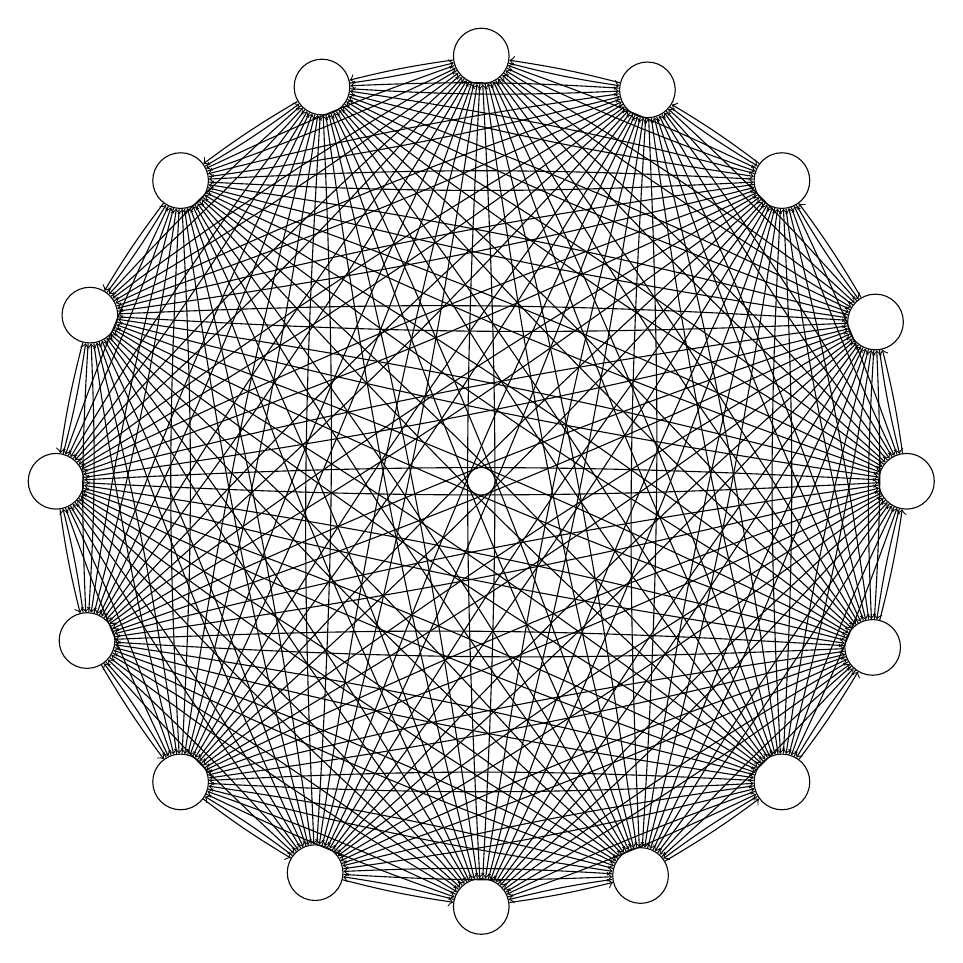
\begin{tikzpicture}[transform shape]
  %the multiplication with floats is not possible. Thus I split the loop in two.
  \foreach \number in {1,...,8}{
      % Computer angle:
        \mycount=\number
        \advance\mycount by -1
  \multiply\mycount by 45
        \advance\mycount by 0
      \node[draw,circle,inner sep=0.25cm] (N-\number) at (\the\mycount:5.4cm) {};
    }
  \foreach \number in {9,...,16}{
      % Computer angle:
        \mycount=\number
        \advance\mycount by -1
  \multiply\mycount by 45
        \advance\mycount by 22.5
      \node[draw,circle,inner sep=0.25cm] (N-\number) at (\the\mycount:5.4cm) {};
    }
  \foreach \number in {1,...,15}{
        \mycount=\number
        \advance\mycount by 1
  \foreach \numbera in {\the\mycount,...,16}{
    \path (N-\number) edge[->,bend right=3] (N-\numbera)  edge[<-,bend
      left=3] (N-\numbera);
  }
}
\end{tikzpicture}


\begin{tikzpicture}
 \definecolor{r1}{RGB}{0,129,188}
 \definecolor{r2}{RGB}{252,177,49}
 \definecolor{r3}{RGB}{35,34,35}
 \definecolor{r4}{RGB}{0,157,87}
 \definecolor{r5}{RGB}{238,50,78}
 \begin{scope}
   \clip (-6,2) rectangle (6,-.9);
   \foreach \col/\xp/\yp in {
     r5/4/0, r4/2/-1.8, r3/0/0,
     r2/-2/-1.8, r1/-4/0
   } {
     \path[draw=white,line width=.08cm,
     fill=\col,even odd rule]
     (\xp, \yp) circle (1.9cm)
     (\xp, \yp) circle (1.5cm);
   }
 \end{scope}
 \begin{scope}
   \clip (-6,-.9) rectangle (6,-3.8);
   \foreach \col/\xp/\yp in {
     r1/-4/0, r2/-2/-1.8, r3/0/0,
     r4/2/-1.8, r5/4/0
   } {
     \path[draw=white,line width=.08cm,
     fill=\col,even odd rule]
     (\xp, \yp) circle (1.9cm)
     (\xp, \yp) circle (1.5cm);
   }
 \end{scope}
\end{tikzpicture}


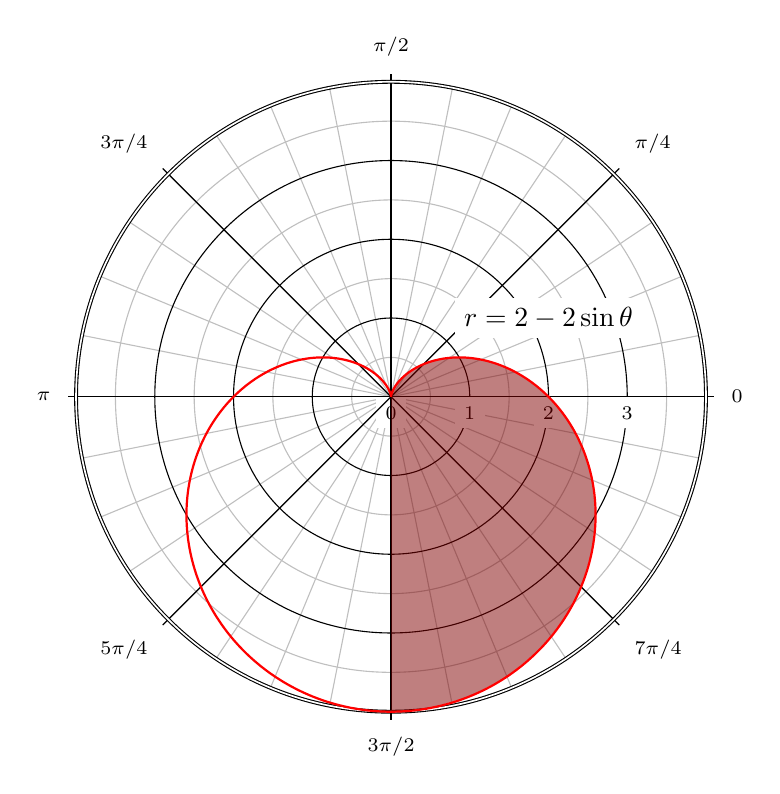
\begin{tikzpicture}[>=latex]

% Draw the lines at multiples of pi/12
\foreach \ang in {0,...,31} {
  \draw [lightgray] (0,0) -- (\ang * 180 / 16:4);
}

% Concentric circles and radius labels
\foreach \s in {0, 1, 2, 3} {
  \draw [lightgray] (0,0) circle (\s + 0.5);
  \draw (0,0) circle (\s);
  \node [fill=white] at (\s, 0) [below] {\scriptsize $\s$};
}

% Add the labels at multiples of pi/4
\foreach \ang/\lab/\dir in {
  0/0/right,
  1/{\pi/4}/{above right},
  2/{\pi/2}/above,
  3/{3\pi/4}/{above left},
  4/{\pi}/left,
  5/{5\pi/4}/{below left},
  7/{7\pi/4}/{below right},
  6/{3\pi/2}/below} {
  \draw (0,0) -- (\ang * 180 / 4:4.1);
  \node [fill=white] at (\ang * 180 / 4:4.2) [\dir] {\scriptsize $\lab$};
}

% The double-lined circle around the whole diagram
\draw [style=double] (0,0) circle (4);

\fill [fill=red!50!black, opacity=0.5] plot [domain=-pi/2:pi/2]
  (xy polar cs:angle=\x r, radius= {2-2*sin(\x r)});
\draw [thick, color=red, domain=0:2*pi, samples=200, smooth]
  plot (xy polar cs:angle=\x r, radius={2-2*sin(\x r)});
\node [fill=white] at (2,1) {$r=2-2\sin\theta$};

\end{tikzpicture} 


% definition de partial ellipse
\tikzset{partial ellipse/.style args =
  {#1:#2:#3}{insert path={+ (#1:#3) arc (#1:#2:#3)}}}
\begin{tikzpicture}[>=latex]
  %  ellipses
  \draw [fill=white!90!red]    (3,-1.8) ellipse    (4cm and 1 cm);
  \draw [fill=yellow!90!green] (3,-1.8) ellipse (3cm and 0.75 cm);
  \draw [fill=white!90!green]  (3,-1.8) ellipse  (2cm and 0.5 cm);

  % -- Soleil
  \shade [ball color=gray!10!yellow] (3,-1.8) circle (1);
  \node (soleil) at (3,-1.8) {\bf Soleil};
  % partial ellipse pour tracé devant le Soleil
  \draw (3,-1.8) [partial ellipse=220:320:2cm and 0.5cm]
        (3,-1.8) [partial ellipse=220:320:3cm and 0.75cm];

  % Venus
  \shade [ball color=gray!10!orange] (1.6,-1.8) circle (.2);
  \node (venus) at (1.5,-1.45) {Venus}; 

  % ombre de Venus
  \draw[color=white!70!black,fill=white!70!black]
    (1.6,-2.3) ellipse (2mm and 0.5mm);

  % Mercure
  \shade [ball color=gray!10!orange] (5,-1.225) circle (.25);
  \node (mercure) at (5,-0.8) {Mercure}; 

  % Earth
  \shade [ball color=white!50!blue] (5.75,-2.5) circle (.33);
  \node (terre) at (6.6,-2.6) {\bf Terre};

  % Lune
  \shade [ball color=yellow] (5.25,-2.8) circle (.1);
  \node (lune) at (5.25,-3) {Lune};
     
  % Mars
  \draw (3,-1.8) [partial ellipse=45:120:9cm and 2.5cm];
  \shade [ball color=black!50!red] (5,0.66) circle (.15);
  \node (mars) at (5,1) {\bf Mars};   
  % trajet
  \draw [line width=2pt,blue,->,>=latex] (terre) to[out=0,in=0] (mars);   
\end{tikzpicture}
\end{center}


\end{document}
